\documentclass[12pt, twoside]{article}
\usepackage[letterpaper, margin=1in, headsep=0.2in]{geometry}
\setlength{\headheight}{0.6in}
%\usepackage[english]{babel}
\usepackage[utf8]{inputenc}
\usepackage{microtype}
\usepackage{amsmath}
\usepackage{amssymb}
%\usepackage{amsfonts}
\usepackage{siunitx} %units in math. eg 20\milli\meter
\usepackage{yhmath} % for arcs, overparenth command
\usepackage{tikz} %graphics
\usetikzlibrary{quotes, angles}
\usepackage{graphicx} %consider setting \graphicspath{{images/}}
\usepackage{parskip} %no paragraph indent
\usepackage{enumitem}
\usepackage{multicol}
\usepackage{venndiagram}

\usepackage{fancyhdr}
\pagestyle{fancy}
\fancyhf{}
\renewcommand{\headrulewidth}{0pt} % disable the underline of the header
\raggedbottom
\hfuzz=2mm %suppresses overfull box warnings

\usepackage{hyperref}

\fancyhead[LE]{\thepage}
\fancyhead[RO]{\thepage \\ Name: \hspace{4cm} \,\\}
\fancyhead[LO]{BECA / Dr. Huson / Geometry\\*  Unit 1: Segments, length, and area\\* 30 Sept 2022}

\begin{document}

\subsubsection*{1.13 Extra problems}
\begin{enumerate}
\item Draw the ray $\overrightarrow{WV}$ with a straight edge (or ruler). Measure $VW$ in centimeters. \par \vspace{0.5cm}
  \begin{center}
    \begin{tikzpicture}
    \draw[fill] (0,0) circle [radius=0.05] node[below]{$V$};
    \draw[fill] (-10:5) circle [radius=0.05] node[below]{$W$};
  \end{tikzpicture}
  \end{center}

\item Draw the ray $\overrightarrow{ST}$ with a straight edge (or ruler). Measure $ST$ in centimeters.\par \vspace{0.5cm}
  \begin{center}
    \begin{tikzpicture}
    \draw[fill] (0,0) circle [radius=0.05] node[below]{$T$};
    \draw[fill] (10:7) circle [radius=0.05] node[below]{$S$};
  \end{tikzpicture}
  \end{center}

\item A flat surface is a(n) $\rule{4cm}{0.15mm}$. \bigskip
  
\item Two line segments or angles of equal measure are $\rule{4cm}{0.15mm}$. \bigskip
\item Use conventional notation to write the names of the ray, line, and segment shown.\\.\\
  \vspace{0.5cm}
  \begin{tikzpicture}
    \draw[->, thick] (0,0)--(3,1.5);
    \draw[fill] (0,0) circle [radius=0.05] node[below]{$G$};
    \draw[fill] (2,1) circle [radius=0.05] node[below]{$H$};
    \node at (-1,0) {(a)};
  \end{tikzpicture}  \hspace{.1cm}
  \begin{tikzpicture}
    \draw[<->, thick] (1,1)--(5,0);
    \draw[fill] (2,0.75) circle [radius=0.05] node[below]{$J$};
    \draw[fill] (4,.25) circle [radius=0.05] node[above]{$K$};
    \node at (0,0) {(b)};
  \end{tikzpicture} \hspace{.25cm}
  \begin{tikzpicture}
    \draw[-, thick] (1,0)--(4,2);
    \draw[fill] (1,0) circle [radius=0.05] node[below]{$L$};
    \draw[fill] (4,2) circle [radius=0.05] node[above left]{$M$};
    \node at (0,0) {(c)};
  \end{tikzpicture}
  \vspace{1cm}

\item Points that are all located on the same plane are $\rule{4cm}{0.15mm}$.\bigskip

\item Two rays with a common vertex compose a(n) $\rule{4cm}{0.15mm}$. \bigskip
\item Points that are all located on the same line are $\rule{4cm}{0.15mm}$.\bigskip

\item Use conventional notation to write the names of the ray, line, and segment shown.\\.\\
  \vspace{0.5cm}
  \begin{tikzpicture}
    \draw[-, thick] (1,0)--(4,2);
    \draw[fill] (1,0) circle [radius=0.05] node[below]{$A$};
    \draw[fill] (4,2) circle [radius=0.05] node[above left]{$B$};
    \node at (0,0) {(a)};
  \end{tikzpicture} \hspace{.25cm}
  \begin{tikzpicture}
    \draw[->, thick] (0,0)--(3,1.5);
    \draw[fill] (0,0) circle [radius=0.05] node[below]{$P$};
    \draw[fill] (2,1) circle [radius=0.05] node[below]{$Q$};
    \node at (-1,0) {(b)};
  \end{tikzpicture}  \hspace{.1cm}
  \begin{tikzpicture}
    \draw[<->, thick] (1,1)--(5,0);
    \draw[fill] (2,0.75) circle [radius=0.05] node[below]{$S$};
    \draw[fill] (4,.25) circle [radius=0.05] node[above]{$T$};
    \node at (0,0) {(c)};
  \end{tikzpicture}

\item Two line segments or angles of equal measure are $\rule{4cm}{0.15mm}$. \bigskip

\item Identify three points in the given plane.\\[0.25in]
  \begin{tikzpicture}
    \draw[thick](0,0) node[above right]{$\ p$} --(6,0)--(8,4)--(2,4)--(0,0);
    \draw[<->, thick] (1,1)--(6,3);
    \draw[fill] (3.5,2) circle [radius=0.05] node[below]{$W \ $};
    \draw[fill] (5,2.6) circle [radius=0.05] node[below]{$X$};
    \draw[<->, thick] (2,3.5)--(5.25,.25);
    \draw[fill] (5,0.5) circle [radius=0.05] node[below left]{$Y$};
  \end{tikzpicture} \vspace{1cm}
  
\item Identify two line segments in the given plane.\\[0.25in]
  \begin{tikzpicture}
    \draw[thick](0,0) node[above right]{$\ p$} --(6,0)--(8,4)--(2,4)--(0,0);
    \draw[<->, thick] (1,1)--(6,3);
    \draw[fill] (3.5,2) circle [radius=0.05] node[below]{$J \ $};
    \draw[fill] (5,2.6) circle [radius=0.05] node[below]{$K$};
    \draw[<->, thick] (2,3.5)--(5.25,.25);
    \draw[fill] (5,0.5) circle [radius=0.05] node[below left]{$L$};
  \end{tikzpicture} \vspace{1cm}
  
\item Given isosceles $\triangle XYZ$ with $\overline{XY} \cong \overline{XZ}$. On the diagram mark the congruent line segments with tick marks.
  \begin{center}
  \begin{tikzpicture}[scale=0.3]
    \draw[thick](0,0)--(9,0)--(4,8)--(0,0);
    \draw[fill] (0,0) circle [radius=0.05] node[below]{$X$};
    \draw[fill] (9,0) circle [radius=0.05] node[below]{$Y$};
    \draw[fill] (4,8) circle [radius=0.05] node[above right]{$Z$};
  \end{tikzpicture}
  \end{center}

\item Given isosceles $\triangle ABC$ with $\overline{AB} \cong \overline{AC}$. On the diagram mark the congruent line segments with tick marks.
\begin{center}
\begin{tikzpicture}[scale=0.3]
  \draw[thick](0,0)--(9,0)--(4,8)--(0,0);
  \draw[fill] (0,0) circle [radius=0.05] node[below]{$A$};
  \draw[fill] (9,0) circle [radius=0.05] node[below]{$B$};
  \draw[fill] (4,8) circle [radius=0.05] node[above right]{$C$};
\end{tikzpicture}
\end{center}

\newpage   
\item Given $\overline{ABC}$, $AB=29$, and $BC=63$. 
  Find ${AC}$.
  \begin{flushright}
    \begin{tikzpicture}
      \draw[-, thick] (0,0)--(6,0);
      \draw[fill] (0,0) circle [radius=0.05] node[below]{$A$};
      \draw[fill] (2,0) circle [radius=0.05] node[below]{$B$};
      \draw[fill] (6,0) circle [radius=0.05] node[below]{$C$};
    \end{tikzpicture} \vspace{2cm}
  \end{flushright}
  \item Given $\overline{ABC}$, $AB=84$, and $AC=116$. 
  Find ${BC}$.
  \begin{flushright}
    \begin{tikzpicture}
      \draw[-, thick] (1,0)--(7,0);
      \draw[fill] (1,0) circle [radius=0.05] node[below]{$A$};
      \draw[fill] (5,0) circle [radius=0.05] node[below]{$B$};
      \draw[fill] (7,0) circle [radius=0.05] node[below]{$C$};
    \end{tikzpicture}
  \end{flushright}

\item Given $\overline{DEF}$, $DE=7 \frac{1}{3}$, and $EF=3 \frac{1}{6}$.
  Find ${DF}$.
  \begin{flushright}
    \begin{tikzpicture}
      \draw[-, thick] (1,0)--(7,0);
      \draw[fill] (1,0) circle [radius=0.05] node[below]{$D$};
      \draw[fill] (5,0) circle [radius=0.05] node[below]{$E$};
      \draw[fill] (7,0) circle [radius=0.05] node[below]{$F$};
    \end{tikzpicture}
  \end{flushright}

\item Given $\overline{DEF}$, $DE=5 \frac{1}{14}$, and $DF=9 \frac{4}{7}$.
  Find ${EF}$. State as a fraction. \vspace{1cm}
  \begin{flushright}
    \begin{tikzpicture}
      \draw[-, thick] (0,0)--(6,0);
      \draw[fill] (0,0) circle [radius=0.05] node[below]{$D$};
      \draw[fill] (3.5,0) circle [radius=0.05] node[below]{$E$};
      \draw[fill] (6,0) circle [radius=0.05] node[below]{$F$};
    \end{tikzpicture} \vspace{1cm}
  \end{flushright}

\item Find the distance between $M$ and $N$. 
\begin{flushright}
    \begin{tikzpicture}
      \draw[<->] (-5.5,0)--(4.5,0);
      \foreach \x in {-5,...,4}
        \draw[shift={(\x,0)},color=black] (0pt,-3pt) -- (0pt,3pt) node[below=5pt]  {$\x$};
        \draw[fill] (-4,0) circle [radius=0.05] node[above] {$M(-4)$};
        \draw[fill] (3,0) circle [radius=0.05] node[above] {$N(3)$};
    \end{tikzpicture}
  \end{flushright} \vspace{0.75cm}  

\item Find the distance between $P$ and $Q$. 
\begin{flushright}
    \begin{tikzpicture}
      \draw[<->] (-4.5,0)--(5.5,0);
      \foreach \x in {-4,...,5}
        \draw[shift={(\x,0)},color=black] (0pt,-3pt) -- (0pt,3pt) node[below=5pt]  {$\x$};
        \draw[fill] (-2,0) circle [radius=0.05] node[above] {$P(-2)$};
        \draw[fill] (4,0) circle [radius=0.05] node[above] {$Q(4)$};
    \end{tikzpicture}
  \end{flushright} \vspace{0.75cm}  

\item Find $RS$, given $R=0.7$ and $S=5.3$.
\begin{flushright}
  \begin{tikzpicture}
    \draw[<->] (-1.5,0)--(6.5,0);
    \foreach \x in {-1,...,6}
      \draw[shift={(\x,0)},color=black] (0pt,-3pt) -- (0pt,3pt) node[below=5pt]  {$\x$};
      \draw[fill] (0.7,0) circle [radius=0.05] node[above] {$R$};
      \draw[fill] (5.3,0) circle [radius=0.05] node[above] {$S$};
  \end{tikzpicture}
\end{flushright}

\item Find $GH$, given $G=1.4$ and $H=6.1$.
\begin{flushright}
  \begin{tikzpicture}
    \draw[<->] (-1.5,0)--(7.5,0);
    \foreach \x in {-1,...,7}
      \draw[shift={(\x,0)},color=black] (0pt,-3pt) -- (0pt,3pt) node[below=5pt]  {$\x$};
      \draw[fill] (1.4,0) circle [radius=0.05] node[above] {$G$};
      \draw[fill] (6.1,0) circle [radius=0.05] node[above] {$H$};
  \end{tikzpicture}
\end{flushright} \vspace{1.75cm}

\item Given $\overline{ABC}$, $AB=\frac{2}{3}$, and $AC=3 \frac{1}{3}$. \par \smallskip
  Find ${BC}$. \par \smallskip
  \begin{tikzpicture}
    \draw[thick] (1,0)--(7,0);
    \draw[fill] (1,0) circle [radius=0.05] node[below]{$A$};
    \draw[fill] (2,0) circle [radius=0.05] node[below]{$B$};
    \draw[fill] (7,0) circle [radius=0.05] node[below]{$C$};
  \end{tikzpicture} \vspace{1cm}

\item Given $\overline{DEFG}$, $DE=3 \frac{1}{4}$, $EF=6 \frac{1}{4}$, and $FG= 1 \frac{3}{4}$. (diagram not to scale) \par \smallskip
Find ${DG}$, expressed as a fraction, not a decimal. \vspace{1cm}
  \begin{flushleft}
    \begin{tikzpicture}
      \draw[thick] (0,0)--(9,0);
      \draw[fill] (0,0) circle [radius=0.05] node[below]{$D$};
      \draw[fill] (3,0) circle [radius=0.05] node[below]{$E$};
      \draw[fill] (7,0) circle [radius=0.05] node[below]{$F$};
      \draw[fill] (9,0) circle [radius=0.05] node[below]{$G$};
    \end{tikzpicture}
  \end{flushleft} \vspace{1cm}
  
\item Given $\overline{FGHI}$, $FG=8 \frac{1}{6}$, $GH=12 \frac{1}{3}$, and $HI= 5 \frac{1}{2}$. (diagram not to scale) \par \smallskip
Find ${FI}$. \par \bigskip
  \begin{tikzpicture}
    \draw[thick] (0,0)--(9,0);
    \draw[fill] (0,0) circle [radius=0.05] node[below]{$F$};
    \draw[fill] (3,0) circle [radius=0.05] node[below]{$G$};
    \draw[fill] (7,0) circle [radius=0.05] node[below]{$H$};
    \draw[fill] (9,0) circle [radius=0.05] node[below]{$I$};
  \end{tikzpicture} \vspace{1cm}

\item Given $\overleftrightarrow{JK}$ as shown on the number line. \par \smallskip
  \begin{tikzpicture}[scale=0.5]
    \draw[<->] (49,0)--(71,0);
    \foreach \x in {50, 52,...,70}
      \draw[shift={(\x,0)}] (0pt,-6pt)--(0pt,6pt) node[below=5pt]{$\x$};
    \draw[fill] (54,0) circle [radius=0.1] node[above]{$J$};
    \draw[fill] (68,0) circle [radius=0.1] node[above]{$K$};
  \end{tikzpicture} \par \bigskip
  What is the midpoint between the points $J$ and $K$? \vspace{2cm}

\item The point $M(2.3)$ is the midpoint of segment $\overline{AB}$. Given $A(-1.5)$, find the value of $B$. Mark and label it below. \par \smallskip
\begin{tikzpicture}
  \draw[<->] (-2.5,0)--(8.5,0);
  \foreach \x in {-2,...,8}
    \draw[shift={(\x,0)}] (0pt,-3pt)--(0pt,3pt) node[below=5pt]{$\x$};
  \draw[fill] (-1.5,0) circle [radius=0.05] node[above]{$A(-1.5)$};
  \draw[fill] (2.3,0) circle [radius=0.05] node[above]{$M(2.3)$};
\end{tikzpicture} \vspace{1cm}

\item Given $\overleftrightarrow{RS}$ as shown on the number line, with $R=-2.8$ and $S=4.4$. \par \smallskip
  \begin{tikzpicture}
    \draw[<->] (-4.5,0)--(6.5,0);
    \foreach \x in {-4,...,6} %2 leading for diff!=1
      \draw[shift={(\x,0)},color=black] (0pt,-3pt) -- (0pt,3pt) node[below=5pt]  {$\x$};
      \draw[fill] (-2.8,0) circle [radius=0.05] node[above]{$R$};
      \draw[fill] (4.4,0) circle [radius=0.05] node[above]{$S$};
  \end{tikzpicture} \par \smallskip
  The points $T$ and $U$ trisect $\overline{RS}$. Find their values, and mark and label them on the number line. \vspace{1cm}

\item Given $\overline{ABC}$, $AB=84$, $AC=116$.\\ [0.25cm]
  Find ${BC}$.\\[1.5cm]
  \begin{tikzpicture}
    \draw[-, thick] (1,0)--(7,0);
    \draw[fill] (1,0) circle [radius=0.05] node[below]{$A$};
    \draw[fill] (5,0) circle [radius=0.05] node[below]{$B$};
    \draw[fill] (7,0) circle [radius=0.05] node[below]{$C$};
  \end{tikzpicture} \vspace{2cm}

\item Given $\overline{DEF}$, $DE=3 \frac{1}{3}$, and $EF=4 \frac{1}{6}$. \\ [0.25cm]
  Find ${DF}$.\\[1.5cm]
    \begin{tikzpicture}[scale=0.8]
      \draw[-, thick] (0,0)--(7,0);
      \draw[fill] (0,0) circle [radius=0.05] node[below]{$D$};
      \draw[fill] (3,0) circle [radius=0.05] node[below]{$E$};
      \draw[fill] (7,0) circle [radius=0.05] node[below]{$F$};
    \end{tikzpicture} \vspace{2cm}


\item Given $\overline{DEFG}$, $DE=3 \frac{1}{4}$, $EF=6 \frac{1}{4}$, and $FG= 1 \frac{3}{4}$. (diagram not to scale)\\ [0.25cm]
Find ${DG}$, expressed as a fraction, not a decimal.
  \begin{flushright}
    \begin{tikzpicture}
      \draw[-, thick] (0,0)--(9,0);
      \draw[fill] (0,0) circle [radius=0.05] node[below]{$D$};
      \draw[fill] (3,0) circle [radius=0.05] node[below]{$E$};
      \draw[fill] (7,0) circle [radius=0.05] node[below]{$F$};
      \draw[fill] (9,0) circle [radius=0.05] node[below]{$G$};
    \end{tikzpicture}
  \end{flushright}

\item Given $\overline{DEFG}$, $DE=3 \frac{1}{4}$, $EF=6 \frac{1}{4}$, and $FG= 1 \frac{3}{4}$. (diagram not to scale)\\ [0.25cm]
  Find ${DG}$, expressed as a fraction, not a decimal.
  \begin{flushright}
      \begin{tikzpicture}
        \draw[-, thick] (0,0)--(9,0);
        \draw[fill] (0,0) circle [radius=0.05] node[below]{$D$};
        \draw[fill] (3,0) circle [radius=0.05] node[below]{$E$};
        \draw[fill] (7,0) circle [radius=0.05] node[below]{$F$};
        \draw[fill] (9,0) circle [radius=0.05] node[below]{$G$};
      \end{tikzpicture}
    \end{flushright}

\item Given $P(-2.4)$ and $Q(1.8)$, as shown on the number line. \\[0.25cm]
  Find the length of the line segment $\overline{PQ}$. State an equation for full credit.
  \begin{center}
    \begin{tikzpicture}
      \draw[<->] (-4.5,0)--(4.5,0);
      \draw[-, thick] (-2.4,0)--(1.8,0);
      \foreach \x in {-4,...,4} %2 leading for diff!=1
        \draw[shift={(\x,0)},color=black] (0pt,-3pt) -- (0pt,3pt) node[below=5pt]  {$\x$};
        \draw[fill] (-2.4,0) circle [radius=0.05] node[above] {$P$};
        \draw[fill] (1.8,0) circle [radius=0.05] node[above] {$Q$};
    \end{tikzpicture}
  \end{center}

\item Given $P(-2.4)$ and $Q(1.8)$, as shown on the number line. \\[0.25cm]
Find the length of the line segment $\overline{PQ}$. State an equation for full credit.
  \begin{center}
    \begin{tikzpicture} 
      \draw[<->] (-4.5,0)--(4.5,0);
      \draw[-, thick] (-2.4,0)--(1.8,0);
      \foreach \x in {-4,...,4} %2 leading for diff!=1
        \draw[shift={(\x,0)},color=black] (0pt,-3pt) -- (0pt,3pt) node[below=5pt]  {$\x$};
        \draw[fill] (-2.4,0) circle [radius=0.05] node[above] {$P$};
        \draw[fill] (1.8,0) circle [radius=0.05] node[above] {$Q$};
    \end{tikzpicture}
  \end{center}

\item Given $\overleftrightarrow{PQ}$ as shown on the number line. Find $PQ$. \\[20pt] % Midpoint
  \begin{tikzpicture}
    \draw[<->] (-4.5,0)--(6.5,0);
    \foreach \x in {-4,...,6} %2 leading for diff!=1
      \draw[shift={(\x,0)},color=black] (0pt,-3pt) -- (0pt,3pt) node[below=5pt]  {$\x$};
      \draw[fill] (-2,0) circle [radius=0.05] node[above] {$P$};
      \draw[fill] (4,0) circle [radius=0.05] node[above] {$Q$};
  \end{tikzpicture} \\ \bigskip
  \vspace{1cm}  
  
\item Given $\overleftrightarrow{RS}$, with $R=0.7$ and $S=5.3$. Find $RS$, showing the formula.\\[20pt]
    \begin{tikzpicture}
      \draw[<->] (-4.5,0)--(6.5,0);
      \foreach \x in {-4,...,6} %2 leading for diff!=1
        \draw[shift={(\x,0)},color=black] (0pt,-3pt) -- (0pt,3pt) node[below=5pt]  {$\x$};
        \draw[fill] (0.7,0) circle [radius=0.05] node[above] {$R$};
        \draw[fill] (5.3,0) circle [radius=0.05] node[above] {$S$};
    \end{tikzpicture} \\ \bigskip

\item Given $\overline{DEFG}$, $DE=3 \frac{1}{4}$, $EF=6 \frac{1}{4}$, and $FG= 1 \frac{3}{4}$. (diagram not to scale)\\ [0.25cm]
  Find ${DG}$, expressed as a fraction, not a decimal.
  \begin{flushright}
      \begin{tikzpicture}
        \draw[-, thick] (0,0)--(9,0);
        \draw[fill] (0,0) circle [radius=0.05] node[below]{$D$};
        \draw[fill] (3,0) circle [radius=0.05] node[below]{$E$};
        \draw[fill] (7,0) circle [radius=0.05] node[below]{$F$};
        \draw[fill] (9,0) circle [radius=0.05] node[below]{$G$};
      \end{tikzpicture}
    \end{flushright}

\item Given $P(-2.4)$ and $Q(1.8)$, as shown on the number line. \\[0.25cm]
  Find the length of the line segment $\overline{PQ}$. State an equation for full credit.
  \begin{center}
    \begin{tikzpicture}
      \draw[<->] (-4.5,0)--(4.5,0);
      \draw[-, thick] (-2.4,0)--(1.8,0);
      \foreach \x in {-4,...,4} %2 leading for diff!=1
        \draw[shift={(\x,0)},color=black] (0pt,-3pt) -- (0pt,3pt) node[below=5pt]  {$\x$};
        \draw[fill] (-2.4,0) circle [radius=0.05] node[above] {$P$};
        \draw[fill] (1.8,0) circle [radius=0.05] node[above] {$Q$};
    \end{tikzpicture}
  \end{center}

\item Given $\overline{PQR}$, $PQ=3x+14$, $QR=2x+5$, $PR=4x+28$. \\[0.5cm]
Write down an equation to represent the situation.
  \begin{center}
    \begin{tikzpicture}
    \draw[-, thick] (0,0)--(7,0);
    \draw[fill] (0,0) circle [radius=0.05] node[below]{$P$};
    \draw[fill] (5,0) circle [radius=0.05] node[below]{$Q$};
    \draw[fill] (7,0) circle [radius=0.05] node[below]{$R$};
    \node at (2,0) [above]{$3x+14$};
    \node at (6,0) [above]{$2x+5$};
    \draw[<->, dashed] (0,-0.7)--(7,-0.7);
    \node at (3.5,-0.7) [below]{$4x+28$};
  \end{tikzpicture}
  \end{center}
        
\item Given $\overline{PQRS}$. $Q$ is the midpoint of $\overline{PS}$, and $R$ bisects $\overline{QS}$. \\[0.5cm] 
If $PR= 4 \frac{1}{2}$ find ${PS}$. Justify your answer.
  \begin{flushright}
      \begin{tikzpicture}
        \draw[-, thick] (0,0)--(8,0);
        \draw[fill] (0,0) circle [radius=0.05] node[below]{$P$};
        \draw[fill] (4,0) circle [radius=0.05] node[below]{$Q$};
        \draw[fill] (6,0) circle [radius=0.05] node[below]{$R$};
        \draw[fill] (8,0) circle [radius=0.05] node[below]{$S$};
      \end{tikzpicture}
    \end{flushright}

\item Given $A(0)$ and $T(2)$, as shown on the number line. $T$ is one of the points that trisects $\overline{AB}$.  \\[0.25cm]
  Find $B$. For full credit, find both solutions.
  \begin{center}
    \begin{tikzpicture}
      \draw[<->] (-2.5,0)--(7.5,0);
      %\draw[-, thick] (0,0)--(2,0);
      \foreach \x in {-2,...,7} %2 leading for diff!=1
        \draw[shift={(\x,0)},color=black] (0pt,-3pt) -- (0pt,3pt) node[below=5pt]  {$\x$};
        \draw[fill] (0,0) circle [radius=0.05] node[above] {$A$};
        \draw[fill] (2,0) circle [radius=0.05] node[above] {$T$};
    \end{tikzpicture}
  \end{center}

\item Given $\overline{DEFG}$, $DE=1 \frac{2}{5}$, $EF=2 \frac{3}{10}$, and $FG= \frac{4}{5}$. (diagram not to scale)\\ [0.25cm]
  Find ${DG}$, expressed as a fraction, not a decimal.
  \begin{flushright}
    \begin{tikzpicture}
      \draw[-, thick] (0,0)--(9,0);
      \draw[fill] (0,0) circle [radius=0.05] node[below]{$D$};
      \draw[fill] (3,0) circle [radius=0.05] node[below]{$E$};
      \draw[fill] (7,0) circle [radius=0.05] node[below]{$F$};
      \draw[fill] (9,0) circle [radius=0.05] node[below]{$G$};
    \end{tikzpicture}
    \end{flushright}
  
\item Given $M$ is the midpoint of $\overline{AB}$, $AM=7x+1$, $MB=33-x$.
  \begin{enumerate}
    \item Mark the diagram with the values and tick marks
    \item Write an equation that could be solved for $x$
  \end{enumerate} \vspace{1cm}
  \begin{center}
    \begin{tikzpicture}
      \draw[fill] (0,0) circle [radius=0.05] node[below]{$A$};
      \draw[-, thick] (0,0)--(7,0);
      \draw[fill] (3.5,0) circle [radius=0.05] node[below]{$M$};
      \draw[fill] (7,0) circle [radius=0.05] node[below]{$B$};
      %\node at (1.7,0.5) [above]{$x+2$};
      %\node at (5.2,0.5) [above]{$11$};
      %\draw[<->, dashed] (0,-1)--(7,-1);
      %\node at (3.5,-1) [below]{$20$};
    \end{tikzpicture}
  \end{center}

\item Given points on the number line $E(1.2)$ and $G(5.6)$ as shown. Find the midpoint $F$ of $\overline{EG}$. Mark it on the number line and label it as an ordered pair.\\[20pt]
  \begin{tikzpicture}
    \draw[<->] (-2.5,0)--(6.5,0);
    \foreach \x in {-2,...,6} %2 leading for diff!=1
      \draw[shift={(\x,0)},color=black] (0pt,-3pt) -- (0pt,3pt) node[below=5pt]  {$\x$};
    \draw[thick] (1.2,0)--(5.6,0);
    \draw[fill] (1.2,0) circle [radius=0.05] node[above] {$E(1.2)$};
    \draw[fill] (5.6,0) circle [radius=0.05] node[above] {$G(5.6)$};
  \end{tikzpicture}

\item The horizontal line segment $\overline{RS}$ is plotted on the coordinate plane with $R(2,3)$ and $S(7,3)$. 
\begin{multicols}{2}
  Find length $RS$, showing the calculation.
    \begin{flushright}
    \begin{tikzpicture}[scale=.635]
      \draw[help lines] (-1,-1) grid (9,6);
      \draw[thick, ->] (-1.2,0) -- (9.4,0) node [below right] {$x$};
      \draw[thick, ->] (0,-1.2)--(0,6.4) node [left] {$y$};
      \draw[-, thick] (2,3)--(7,3);
      \draw[fill] (2,3) circle [radius=0.05] node[below]{$R(2,3)$};
      \draw[fill] (7,3) circle [radius=0.05] node[below right]{$S(7,3)$};
    \end{tikzpicture}
    \end{flushright}
\end{multicols} 

\item The vertical line segment $\overline{PQ}$ is plotted on the coordinate plane with $P(3,5)$ and $Q(3,1)$. 
\begin{multicols}{2}
  Find the length $PQ$. \\[0.5cm]
  Show the calculation, including the absolute value bars.
    \begin{flushright}
    \begin{tikzpicture}[scale=.635]
      %\draw[help lines] (-1,-1) grid (9,9);
      \draw[thick, ->] (-1.2,0) -- (9.4,0) node [below right] {$x$};
      \draw[thick, ->] (0,-1.2)--(0,7.4) node [left] {$y$};
      \draw[-, thick] (3,5)--(3,1);
      \draw[fill] (3,5) circle [radius=0.05] node[right]{$P(3,5)$};
      \draw[fill] (3,1) circle [radius=0.05] node[right]{$Q(3,1)$};
    \end{tikzpicture}
    \end{flushright}
\end{multicols}
  
\newpage
\subsubsection*{Do Not Solve! Make a drawing on the right, an equation to the left, and circle where it states what to find.}
  \vspace{0.5cm}
\item The point $Q$ is the midpoint of $\overline{PR}$, $PQ=11$, and $QR=2x+1$. Find ${x}$.
\item Given $\overline{PQR}$, with $PQ=3x-7$, $QR=x+3$, and $PR=12$. Find ${x}$.
\item Given that $Q$ bisects $\overline{PR}$. $PQ=2x-5$, $PR=42$. Find ${x}$.
\item The points $P$, $Q$, and $R$ are collinear, with $PQ=x+4$ and $PR=27$. $\overline{QR}$ is twice the length of $\overline{PQ}$. Find ${x}$.

\subsubsection*{Do Not Solve! Draw and label the situation on the right, model with an equation to the left, and circle where it states what to find.}
  \vspace{0.5cm}

\item Given $\overline{ABC}$, with $AB=2x-7$, $BC=3x-3$, and $AC=15$. Find ${AB}$.
\item Given that $K$ bisects $\overline{JL}$. $JK=3x+8$, $KL=17$. Find ${x}$.
\item The point $M$ is the midpoint of $\overline{UV}$, $UM=x+7$, and $MV=2x+1$. Find ${UV}$.
\item The points $P$, $Q$, and $R$ are collinear, with $PQ=6x+16$ and $PR=42$. $\overline{QR}$ is half the length of $\overline{PQ}$. Find ${x}$.

\newpage
\item Given isosceles $\triangle ABC$ with $\overline{AC} \cong \overline{BC}$. $AC=5x+7$ and $BC=3x+17$. \\ Find $AC$.\\[0.5cm]
  \begin{tikzpicture}[scale=0.55]
    \draw[thick](0,0)--(4,0)--(2,6)--(0,0);
    \draw[fill] (0,0) circle [radius=0.05] node[below]{$A$};
    \draw[fill] (4,0) circle [radius=0.05] node[below]{$B$};
    \draw[fill] (2,6) circle [radius=0.05] node[above right]{$C$};
    \draw[thick] (0.8,3)--(1.2,3); %tick mark
    \draw[thick] (2.8,3)--(3.2,3); %tick mark
    \node [right] at (3.25,2.5){$5x+7$};
    \node [left] at (0.75,2.5){$3x+17$};
  \end{tikzpicture}

\item The isosceles $\triangle FGH$ is shown with $\overline{FH} \cong \overline{GH}$. Given $GH=2x+15$ and $FH=19$. \\[0.5cm]
  Write an equation that could be used to find $x$.\\[0.25cm]
    \begin{tikzpicture}[scale=0.5]
      \draw[thick](0,0)--(4,0)--(2,6)--(0,0);
      \draw[fill] (0,0) circle [radius=0.05] node[below left]{$F$};
      \draw[fill] (4,0) circle [radius=0.05] node[below right]{$G$};
      \draw[fill] (2,6) circle [radius=0.05] node[above right]{$H$};
      \draw[thick] (0.8,3.1)--(1.2,3); %tick mark
      \draw[thick] (2.8,3)--(3.2,3.1); %tick mark
      \node at (3.5,3.4) [right]{$2x+15$};
      \node at (0.8,3.4) [left]{$19$};
    \end{tikzpicture}
 
\item The perimeter of the isosceles $\triangle FGH$ is 115 and $\overline{FH} \cong \overline{GH}$. Given $FG=5x+16$ and $FH=34 \frac{1}{2}$. \\[0.5cm]
Write an equation that could be used to find $x$.\\[0.25cm]
  \begin{tikzpicture}[scale=0.5]
    \draw[thick](0,0)--(8,0)--(4,4)--(0,0);
    \draw[fill] (0,0) circle [radius=0.05] node[below left]{$F$};
    \draw[fill] (8,0) circle [radius=0.05] node[below right]{$G$};
    \draw[fill] (4,4) circle [radius=0.05] node[above right]{$H$};
    \draw[thick] (1.8,2.3)--(2.4,1.9); %tick mark
    \draw[thick] (5.6,1.9)--(6.2,2.3); %tick mark
    \node at (4,0) [below]{$5x+16$};
    \node at (1.6,3) [left]{$34 \frac{1}{2}$};
  \end{tikzpicture}
  
\newpage
\item Given the rectangle $ABCD$ shown below, with $AB=6 \frac{1}{3}$ and $BC=2 \frac{1}{2}$. Find the area of the rectangle, expressing your result as a fraction.
  \begin{flushright}
  \begin{tikzpicture}[scale=1.25]
    \draw[-, thick] (0,0)--(4.5,0)--(4.5,2)--(0,2)--cycle;
    \draw[fill] (0,0) circle [radius=0.05] node[left]{$A$};
    \draw[fill] (4.5,0) circle [radius=0.05] node[right]{$B$};
    \draw[fill] (4.5,2) circle [radius=0.05] node[right]{$C$};
    \draw[fill] (0,2) circle [radius=0.05] node[left]{$D$};
    \node at (5, 1){$2 \frac{1}{2}$};
    \node at (2.25, -0.5){$6 \frac{1}{3}$};
  \end{tikzpicture}
  \end{flushright}

\item A triangle has an area of 68 square centimeters. Its height is 16 centimeters. Find the length of its base. \vspace{1cm}

\item A triangle has an area of 75 square centimeters. Its height is 12 centimeters. Find the length of its base. \vspace{1cm}

\item The rectangle $BECA$ has an area of 77, with length $BE=11$.
  \begin{enumerate}
    \item Write an equation with the unknown $w$ as the width of the rectangle. 
    \item Solve.
  \end{enumerate}
  \begin{flushright}
  \begin{tikzpicture}
    \draw[thick] (0,0)--(4,0)--(4,3)--(0,3)--cycle;
    \draw[fill] (0,0) circle [radius=0.05] node[left]{$B$};
    \draw[fill] (4,0) circle [radius=0.05] node[right]{$E$};
    \draw[fill] (4,3) circle [radius=0.05] node[right]{$C$};
    \draw[fill] (0,3) circle [radius=0.05] node[left]{$A$};
    \node at (4.5, 1.5){?};
    \node at (2, -0.5){11};
  \end{tikzpicture}
  \end{flushright}

\item Find the area of rectangle $ABCD$ having length $l=12$ and width $w=4 \frac{1}{2}$. Start with a formula of this form, substituting the given values: \\[0.5cm]
  $A = l \times w$
    \begin{flushright}
    \begin{tikzpicture}[scale=0.6] %1.25]
      \draw[thick] (0,0)--(4.5,0)--(4.5,2)--(0,2)--cycle;
      \draw[fill] (0,0) circle [radius=0.05] node[left]{$A$};
      \draw[fill] (4.5,0) circle [radius=0.05] node[right]{$B$};
      \draw[fill] (4.5,2) circle [radius=0.05] node[right]{$C$};
      \draw[fill] (0,2) circle [radius=0.05] node[left]{$D$};
      \node at (5, 1){$4 \frac{1}{2}$};
      \node at (2.25, -0.5){$12$};
      %\node at (2.25, 1){$A = 15$};
    \end{tikzpicture}
    \end{flushright}
  
\item Rectangle $ABCD$ has area $A=15$ and base $b=6$ but unknown height. Write an equation then solve. Start with this form (for the unknown, use $h$, $x$, or $BC$) and state your answer as a fraction: \\[0.5cm]
  $A = b \times h = 15$
    \begin{flushright}
    \begin{tikzpicture}[scale=0.6] %1.25]
      \draw[thick] (0,0)--(4.5,0)--(4.5,2)--(0,2)--cycle;
      \draw[fill] (0,0) circle [radius=0.05] node[left]{$A$};
      \draw[fill] (4.5,0) circle [radius=0.05] node[right]{$B$};
      \draw[fill] (4.5,2) circle [radius=0.05] node[right]{$C$};
      \draw[fill] (0,2) circle [radius=0.05] node[left]{$D$};
      \node at (5, 1){?};
      \node at (2.25, -0.5){$6$};
      \node at (2.25, 1){$A = 15$};
    \end{tikzpicture}
    \end{flushright}
    
\item Find the base of a rectangle with area $A=16.8$ and height $h=4.8$, expressed as a decimal. First write an equation substituting the given values in the area formula.
  \begin{flushright}
  \begin{tikzpicture}[scale=0.6] %1.25]
    \draw[thick] (0,0)--(3,0)--(3,3.5)--(0,3.5)--cycle;
    \node at (3.5, 2){$4.8$};
    \node at (1.5, -0.5){$x$};
    \node at (1.5, 2){$A = 16.8$};
  \end{tikzpicture}
  \end{flushright}

\item Find the length of the base of a rectangle with area $A=80$ and height $h=10$. Start with the form (use $b$ or $x$): \\[0.5cm]
  $A = b \times h = 80$
  \begin{flushright}
  \begin{tikzpicture}[scale=1.25]
    \draw[thick] (0,0)--(3,0)--(3,3.5)--(0,3.5)--cycle;
    \node at (3.5, 2){$10$};
    \node at (1.5, -0.5){$?$};
    \node at (1.5, 2){$80$};
  \end{tikzpicture}
  \end{flushright}      

\item The shape shown below is composed of straight lines and right angles, with some lengths as marked. Find the perimeter of the figure. Show your work.
  \begin{flushright}
  \begin{tikzpicture}[scale=0.5]
    \draw[-, thick] (0,0)--(13,0)--(13,3)--(9,3)--(9,7)--(13,7)--
    (13, 9)--(0,9)--(0,7)--(4,7)--(4,3)--(0,3)--cycle;
    \node at (4.5, 5){3};
    \node at (2, 2.5){3};
    \node at (8.5, 5){3};
    \node at (11, 2.5){3};
    \node at (6.5, -0.5){10};
    \node at (13.5, 1.5){2};
    \node at (13.5, 8){1};
  \end{tikzpicture}
  \end{flushright} 

\item Find the area and perimeter of the shape shown below. Mark the missing side lengths first. All angles are $90^\circ$.\hfill \emph{(not drawn to scale)}
\begin{flushleft}
\begin{tikzpicture}[rotate=-90, scale=0.6] %1.2]
  \draw[thick] (2,0)--(4.5,0)--(4.5,2.5)--(3,2.5)--(3,5)--(2,5)--cycle;
  \node at (5.1, 1.2){6};
  \node at (4, 2.8){5};
  \node at (3.5, -0.5){7};
  \node at (1.4, 2.5){11};
\end{tikzpicture}
\end{flushleft} \vspace{1cm}

\item Find the area and perimeter of the shape shown below. Mark the missing side lengths first. All angles are $90^\circ$.\hfill \emph{(not drawn to scale)}
  \begin{flushleft}
  \begin{tikzpicture}[rotate=90, scale=0.6]
    \draw[thick] (0,0)--(5,0)--(5,2)--(3,2)--(3,6)--(0,6)--cycle;
    \node at (5.5, 1){3};
    \node at (4, 2.5){4};
    \node at (2.5, -0.5){10};
    \node at (-0.5, 3){13};
  \end{tikzpicture}
  \end{flushleft} \vspace{1cm}

\item Find the area $A$ of the shape shown below in terms of unit squares.
  \begin{flushleft}
    \begin{tikzpicture}[scale=0.6]
      \draw[help lines] (-4,-4) grid (5,3);
      \draw[thick, -] (-3,-3)--(4,-3)--(4,2)--(2,2)--(2,0)--(-1,0)--(-1,2)--(-3,2)--cycle;
    \end{tikzpicture}
  \end{flushleft}
 
\item On the grid below, accurately draw and label two adjacent squares, one with a side length of 4 cm, the other with a side length of 3 cm. The grid is in centimeters. \par \medskip
  Find the area $A$ and perimeter $P$ of combined shape.
  \begin{flushleft}
    \begin{tikzpicture}[scale=0.2]
      \draw[help lines] (-4,-3) grid (5,3);
      %\draw[thick, ->] (-2.2,0) -- (10.4,0) node [below right]{$x$};
      %\draw[thick, ->] (0,-2.2)--(0,10.4) node [left]{$y$};
      %\draw (0,0) circle [radius=3] node[below]{$C$};
      %\draw[fill] (0,0) circle [radius=0.05];
      %\draw[thick, -] (-3,-3)--(4,-3);
    \end{tikzpicture}
  \end{flushleft}
    
\item On the graph, draw polygon ABCDEF with vertices A(1, 1), B(1, 4), C(3, 4), D(3, 7), E(8, 7), and F(8, 1). Find the perimeter and the area of the polygon.
  \begin{flushleft}
    \begin{tikzpicture}[scale=.2]
      \draw[help lines] (0,0) grid (10,10);
      \draw[thick, ->] (0,0) -- (10.4,0) node [below right]{$x$};
      \draw[thick, ->] (0,0)--(0,10.4) node [right]{$y$};
      \foreach \x in {1,...,10}
        \draw[shift={(\x,0)}] (0pt,-3pt)--(0pt,3pt) node[below=5pt]{$\x$};
      \foreach \y in {1,...,10}
        \draw[shift={(0,\y)}] (-3pt,0pt)--(3pt,0pt) node[left=5pt]{$\y$};
    \end{tikzpicture}
    \end{flushleft}
    
\item Draw and label a triangle $\triangle ABC$ with base $\overline{AB}$ 8 centimeters long and altitude of 5 centimeters. (show the altitude as a dotted line, and make sure it is perpendicular to the base) 
  
\newpage
\item Find the area of $\triangle ABC$ shown below (not actual size) with $m\angle C=90^\circ$ and the lengths of the triangle's sides as $a=3$, $b=4$, and $c=5$. 
  \begin{flushright}
  \begin{tikzpicture}[scale=1.4]
    \draw[thick]
    (0,0)node[left]{$A$}--
    (4,0)node[below right]{$C$}--
    (4,2.31)node[right]{$B$}--cycle;
    \draw (4,0)++(-0.3,0)--++(0,0.3)--+(0.3,0);
    \node at (2,0)[below]{$b=4$};
    \node at (4,1.2)[right]{$a=3$};
    \node at (1.8,1.4)[above]{$c=5$};
  \end{tikzpicture}
  \end{flushright}
\vspace{1cm}

\item Find the area of $\triangle ABC$. The altitude $h$ of the triangle is $7$ centimeters and the base $AB=13 \frac{1}{2}$ cm. (diagram not to scale) \par \medskip
\begin{tikzpicture}[scale=1.]
  \draw[thick]
    (2,0)node[below]{$A$}--
    (8,0)node[below]{$B$}--
    (4,3)node[above]{$C$} --(2,0);
 \draw[dashed] (4,0)--(4,3);
 \draw (4,0)++(0.3,0)--++(0,0.3)--+(-0.3,0);
 \node at (4,1.2)[right]{$h=7$};
 \node at (5,0)[below]{$13 \frac{1}{2}$ cm};
\end{tikzpicture}

\item Find the area of $\triangle ABC$. The altitude $h$ of the triangle is $4 \frac{3}{4}$ centimeters and the base $AB=9 \frac{1}{2}$ cm. (diagram not to scale) \par \medskip
  \begin{tikzpicture}[scale=1.]
    \draw[thick]
      (2,0)node[below]{$A$}--
      (8,0)node[below]{$B$}--
      (4,3)node[above]{$C$} --(2,0);
    \draw[dashed] (4,0)--(4,3);
    \draw (4,0)++(0.3,0)--++(0,0.3)--+(-0.3,0);
    \node at (4,1.2)[right]{$h=4 \frac{3}{4}$};
    \node at (5,0)[below]{$9 \frac{1}{2}$ cm};
  \end{tikzpicture}

\item Find the area of $\triangle ABC$. The altitude $h$ of the triangle is $7$ centimeters and the base $AB=13 \frac{1}{2}$ cm. (diagram not to scale) \par \medskip
\begin{tikzpicture}[scale=1.]
  \draw[thick]
    (2,0)node[below]{$A$}--
    (8,0)node[below]{$B$}--
    (4,3)node[above]{$C$} --(2,0);
 \draw[dashed] (4,0)--(4,3);
 \draw (4,0)++(0.3,0)--++(0,0.3)--+(-0.3,0);
 \node at (4,1.2)[right]{$h=7$};
 \node at (5,0)[below]{$13 \frac{1}{2}$ cm};
\end{tikzpicture}

\item Find the height of the $\triangle RST$, having an area of $A=117$ and base $RS=9$.
  \begin{multicols}{2}
    Start by substituting values in the area formula: \\[0.5cm]
    $\displaystyle A = \frac{1}{2} bh = 117$ \vspace{2cm}
      \begin{flushright}
      \begin{tikzpicture}[scale=.635]
        %\draw[help lines] (-1,-1) grid (9,6);
        \draw[thick, ->] (-1.2,0) -- (9.4,0) node [below right] {$x$};
        \draw[thick, ->] (0,-1.2)--(0,8.4) node [left] {$y$};
        \draw[<->, thick] (1.5,1)--(1.5,7);
        \draw[thick] (2,1)--(6,1)--(4,7)--cycle;
        \draw[dashed] (6,1)--(8,7)--(4,7);
        \draw[fill] (2,1) circle [radius=0.05] node[below] {$R$};
        \draw[fill] (6,1) circle [radius=0.05] node[below] {$S$};
        \draw[fill] (4,7) circle [radius=0.05] node[above right] {$T$};
        \node at (4,1)[below]{$9$};
        \node at (1.5,4)[left]{$h$};
      \end{tikzpicture}
      \end{flushright}
  \end{multicols}

\item One side of the $\triangle ABC$ has a length $AB=12$. The triangle's area is 60. Find the length of the altitude $h$ of the triangle to vertex $C$ and perpendicular to side $\overline{AB}$. \par
  \begin{tikzpicture}[scale=0.9, rotate=30]
    \draw[thick]
      (2,0)node[below]{$A$}--
      (8,0)node[below]{$B$}--
      (5,3)node[above]{$C$} --(2,0);
    \draw[dashed] (5,0)--(5,3);
    \draw (5,0)++(0.3,0)--++(0,0.3)--+(-0.3,0);
    \node at (5.2,1.5)[right]{$h=?$};
    \node at (5,-0.5)[below left]{$12$};
  \end{tikzpicture}
  
\item Find the area of $\triangle ABC$ shown below (not actual size) with $m\angle C=90^\circ$ and the lengths of the triangle's sides as $a=3$, $b=4$, and $c=5$. 
  \begin{flushright}
  \begin{tikzpicture}[scale=1.4]
    \draw[thick]
    (0,0)node[left]{$A$}--
    (4,0)node[below right]{$C$}--
    (4,2.31)node[right]{$B$}--cycle;
    \draw (4,0)++(-0.3,0)--++(0,0.3)--+(0.3,0);
    \node at (2,0)[below]{$b=4$};
    \node at (4,1.2)[right]{$a=3$};
    \node at (1.8,1.4)[above]{$c=5$};
  \end{tikzpicture}
  \end{flushright}
  \vspace{1cm}
    
\item Find the area of $\triangle ABC$ shown below (not actual size) with $m\angle C=90^\circ$ and the lengths of the triangle's sides as $a=50$, $b=87$, and $c=100$. \par \medskip
  \begin{tikzpicture}[scale=1.4]
    \draw[thick]
    (0,0)node[left]{$A$}--
    (4,0)node[below right]{$C$}--
    (4,2.31)node[right]{$B$}--cycle;
    \draw (4,0)++(-0.3,0)--++(0,0.3)--+(0.3,0);
    \node at (2,0)[below]{$b=87$};
    \node at (4,1.2)[right]{$a=50$};
    \node at (1.8,1.4)[above]{$c=100$};
  \end{tikzpicture}

\newpage
\item A parallelogram is shown on the $x$-$y$ plane having a base $b=4$ and height $h=3$. 
  \begin{multicols}{2}
  Find its area, showing the calculation.
    \begin{flushright}
    \begin{tikzpicture}[scale=.635]
      \draw[help lines] (-1,-1) grid (9,6);
      \draw[thick, ->] (-1.2,0) -- (9.4,0) node [below right]{$x$};
      \draw[thick, ->] (0,-1.2)--(0,6.4) node [left]{$y$};
      \draw[<->, thick] (1.5,1)--(1.5,4);
      \draw[thick] (2,1)--(6,1)--(7,4)--(3,4)--cycle;
      \node at (4,1)[below]{$4$};
      \node at (1.5,2.5)[left]{$3$};
    \end{tikzpicture}
    \end{flushright}
  \end{multicols} 
  
\item The $\triangle ABC$ is shown below with $A(3,1)$, $B(7,1)$, and $C(1,5)$. The length of the base of the triangle is $AB=4$.
\begin{multicols}{2}
  \begin{enumerate}
    \item Find the height $h$.
    \item Find the triangle's area, showing the calculation. \vspace{2cm}
    \end{enumerate}
    \begin{flushright}
    \begin{tikzpicture}[scale=.635]
      \draw[help lines] (-1,-1) grid (9,6);
      \draw[thick, ->] (-1.2,0) -- (9.4,0) node [below right] {$x$};
      \draw[thick, ->] (0,-1.2)--(0,6.4) node [left] {$y$};
      \draw[<->, thick] (0.5,1)--(0.5,5);
      \draw[thick] (3,1)--(7,1)--(1,5)--cycle;
      \draw[dashed] (7,1)--(5,5)--(1,5);
      \draw[fill] (3,1) circle [radius=0.05] node[below] {$A$};
      \draw[fill] (7,1) circle [radius=0.05] node[below] {$B$};
      \draw[fill] (1,5) circle [radius=0.05] node[above right] {$C$};
      \node at (5,1)[below]{$4$};
      \node at (0.5,3)[right]{$h$};
    \end{tikzpicture}
    \end{flushright}
\end{multicols}

\item The $\triangle ABC$ is shown below with $A(2,1)$, $B(7,1)$, and $C(1,5)$. The length of the base of the triangle is $AB=5$.
  \begin{multicols}{2}
    \begin{enumerate}
      \item Find the height $h$.
      \item Find its area, showing the calculation. \vspace{2cm}
      \end{enumerate}
    \begin{flushright}
    \begin{tikzpicture}[scale=.635]
      \draw[help lines] (-1,-1) grid (9,6);
      \draw[thick, ->] (-1.2,0) -- (9.4,0) node [below right]{$x$};
      \draw[thick, ->] (0,-1.2)--(0,6.4) node [left]{$y$};
      \draw[<->, thick] (0.5,1)--(0.5,5);
      \draw[thick] (2,1)--(7,1)--(1,5)--cycle;
      \draw[dashed] (7,1)--(6,5)--(1,5);
      \draw[fill] (2,1) circle [radius=0.05] node[below]{$A$};
      \draw[fill] (7,1) circle [radius=0.05] node[below]{$B$};
      \draw[fill] (1,5) circle [radius=0.05] node[above right]{$C$};
      \node at (4.5,1)[below]{$5$};
      \node at (0.5,3)[right]{$h$};
    \end{tikzpicture}
    \end{flushright}
  \end{multicols} 

\newpage
\item Find the radius and circumference of circle $O$ with diameter $D=15$ centimeters.
  \begin{multicols}{2}
  \raggedcolumns
  \begin{enumerate}
    \item Write down the radius. \vspace{1.2cm}
    \item State the circumference in terms of $\pi$ \vspace{1cm}
    \item Express the circumference as a decimal, rounding to the \emph{nearest hundredth}.
  \end{enumerate}
  \columnbreak
    \begin{tikzpicture}[scale=1]
      \draw (0,0) circle[radius=3];
      \draw[thick] (0:3)--(0,0)--(-3,0);
      \draw[fill] (0,0) circle [radius=0.05] node[below]{$O$};
      \draw (1.5,0) node[below] {$r$};
    \end{tikzpicture}
  \end{multicols}

\item Given circle $O$ with area $A=64 \pi$ square centimeters.
  \begin{multicols}{2}
  \raggedcolumns
  Find the radius of circle, $OP$. Start with the formula \par \smallskip
  $A = \pi r^2 = 64 \pi$ \vspace{1.7cm}
    \begin{tikzpicture}[scale=0.7]
      \draw (0,0) circle[radius=3];
      \draw[thick]
      (0:3) node[right] {$P$}--
      (0,0) node[below] {$O$};
      \draw (1.5,0) node[below] {$?$};
    \end{tikzpicture}
  \end{multicols}

\item Find the area of the given circle $Q$ with radius $r=10$ centimeters.
  \begin{multicols}{2}
  \raggedcolumns
  Start with the formula \par \medskip
  $A = \pi r^2$ 
  \begin{enumerate}
    \item State the area in terms of $\pi$ \vspace{1.7cm}
    \item Now round to the nearest hundredth
  \end{enumerate}
    \begin{tikzpicture}[scale=1]
      \draw (0,0) circle[radius=3];
      \draw[thick]
      (0:3) node[right]{$P$}--
      (0,0) node[below]{$Q$};
      \draw (1.5,0) node[below]{$10$};
    \end{tikzpicture}
  \end{multicols}
  
\newpage
\item Find the area of the shape shown below composed of a rectangle and circular cap. Leave your answer as an exact value in terms of $\pi$.
  \begin{flushright}
  \begin{tikzpicture}[scale=.635]
    \draw[help lines] (-2,-1) grid (8,7);
    \draw[thick, ->] (-2.2,0) -- (8.4,0) node [below right]{$x$};
    \draw[thick, ->] (0,-1.2)--(0,7.4) node [left]{$y$};
    \draw[thick] (1,1)--(7,1)--(7,3)--(1,3)--cycle;
    %\draw[thick] (3,4) arc (90:270:1);
    \draw[thick] (7,3) arc (0:180:3);
  \end{tikzpicture}
  \end{flushright}
    
\item Find the \emph{perimeter} of the shape shown below composed of a rectangle and circular cap. Leave your answer as an exact value in terms of $\pi$.
    \begin{flushright}
    \begin{tikzpicture}[scale=.635]
      \draw[help lines] (-1,-1) grid (7,7);
      \draw[thick, ->] (-1.2,0) -- (7.4,0) node [below right]{$x$};
      \draw[thick, ->] (0,-1.2)--(0,7.4) node [left]{$y$};
      \draw[thick] (1,1)--(5,1)--(5,4)--(1,4)--cycle;
      \draw[thick] (5,4) arc (0:180:2);
    \end{tikzpicture}
    \end{flushright}
      
\item Given the circle $A$ with radius $r=3$. Leave exact answers, in terms of $\pi$.
  \begin{multicols}{2}
    \begin{enumerate}
      \item Find the circumference of circle $A$. \vspace{1cm}
      \item Find the area of the circle.\vspace{2cm}
    \end{enumerate}
    \begin{flushright}
    \begin{tikzpicture}[scale=.9]
      \draw (0,0) circle [radius=3];
      \draw[fill] (0,0) circle [radius=0.05] node[below right]{$A$};
      \draw[thick, -{>[scale=1.5]}] (0,0)--(30:3);
      \node at (2,0.5){$r=3$};
      \clip (0,0) circle [radius=3];
        \draw[help lines] (-4,-4) grid (4,4);
    \end{tikzpicture}
  \end{flushright}
  \end{multicols}

\newpage    
\subsubsection*{Challenge problems}
\item A square is partitioned into two rectangles. The sum of the perimeters of the two rectangles is 36. Find the area of the square.
\begin{flushright}
\begin{tikzpicture}%[scale=.635]
    \draw [thick]  (0,0) rectangle (6,6);
    \draw [thick] (0,4)--(6,4);
\end{tikzpicture}
\end{flushright}


\end{enumerate}
\end{document}